All models in this experiment are trained on \skill{compose} exercises whose chain length is 1, 2, 3 or 4 with equal probability (length 1 is \skill{follow}), and are tested at lengths 1 to 6.
We compare a block of two layers applied once, twice and three times with unshared stacks of four and six layers.
A looped model with $r$ loops and an unshared model with $2r$ layers perform the same number of layer passes, and the looped one has $1/r$ of the transformer-block parameters.

\begin{table}[t]
\centering\small
\begin{tabular}{@{}lccccccccc@{}}
\toprule
& & Layer & & \multicolumn{4}{c}{G1: chain lengths in training} & \multicolumn{2}{c}{G2: longer} \\
\cmidrule(lr){5-8}\cmidrule(lr){9-10}
Model & Params & passes & Seeds & 1 & 2 & 3 & 4 & 5 & 6 \\
\midrule
2 layers $\times$ 1 loop & 113k & 2 & 1 & 100.0 & 24.9 & 24.4 & 22.9 & 21.4 & 22.1 \\
2 layers $\times$ 2 loops & 113k & 4 & 3 & 100.0 {\scriptsize\,3/3} & 100.0 {\scriptsize\,3/3} & 71.9 {\scriptsize\,1/3} & 23.4 {\scriptsize\,0/3} & 22.2 {\scriptsize\,0/3} & 21.8 {\scriptsize\,0/3} \\
2 layers $\times$ 3 loops & 113k & 6 & 1 & 100.0 & 100.0 & 46.7 & 23.2 & 23.0 & 22.3 \\
4 layers, unshared & 213k & 4 & 3 & 100.0 {\scriptsize\,3/3} & 89.3 {\scriptsize\,1/3} & 55.0 {\scriptsize\,1/3} & 31.3 {\scriptsize\,0/3} & 21.6 {\scriptsize\,0/3} & 21.8 {\scriptsize\,0/3} \\
6 layers, unshared & 313k & 6 & 1 & 100.0 & 95.2 & 65.1 & 25.1 & 22.1 & 22.8 \\
\bottomrule
\end{tabular}

\caption{E3: accuracy (\%) on new textbooks by chain length. Where a model has several seeds, the mean is followed by the number of seeds that ended at 95\% or above out of the number run. Guessing levels for lengths 1 to 6: \GuessOne, \GuessTwo, \GuessThree, \GuessFour, \GuessFive{} and \GuessSix\%.}
\label{tab:e3}
\end{table}

\begin{figure}[t]
\centering
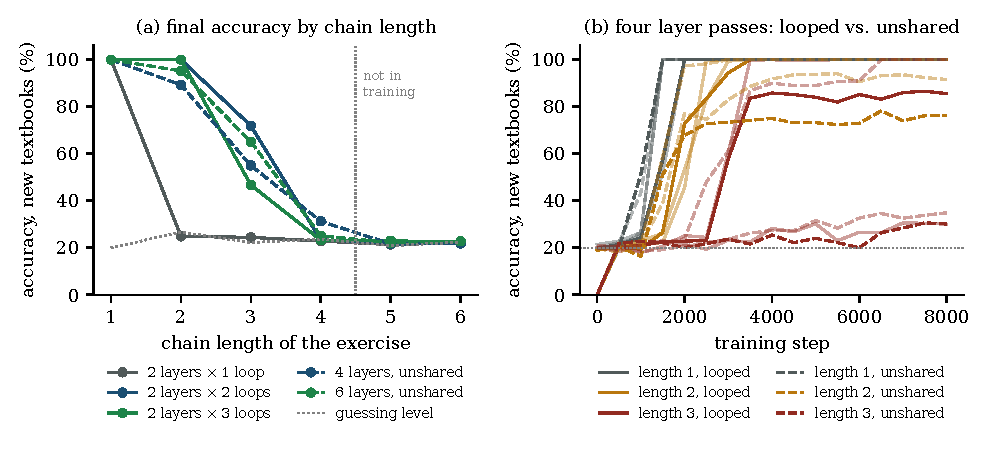
\includegraphics[width=\linewidth]{gen/fig_e3.pdf}
\caption{E3. \textbf{(a)} Final accuracy by chain length, averaged over seeds; solid lines are looped models, dashed lines unshared ones, colour marks the number of layer passes, and the dotted grey curve is the guessing level. \textbf{(b)} Accuracy during training for the two models with four layer passes, one curve per seed (later seeds lighter). The chain lengths are acquired one after another, at times that differ widely between seeds. Dotted horizontal line: 20\%.}
\label{fig:e3}
\end{figure}

\paragraph{Loops supplied depth without adding parameters.}
With two layer passes the model learned single look-ups and nothing longer (\EThreeTiedTwoXOneDepthTwo\% at length 2, below the guessing level; one seed).
Applying the same two layers a second time, with not one parameter added, was enough for length 2 to be solved in all \EThreeTiedTwoXTwoSeeds{} seeds and for length 3 to reach \EThreeTiedTwoXTwoDepthThree\% on average (per seed: \EThreeTiedTwoXTwoDepthThreeList).
This is hypothesis H4 as stated in Section~\ref{sec:protocol}: at a fixed parameter count, a second loop raised the chain length the model could follow.

\paragraph{At equal depth, looped and unshared models showed no consistent difference.}
The unshared four-layer model has the same number of layer passes as the two-loop model and \EThreeUntiedFourParams{} parameters instead of \EThreeTiedTwoXTwoParams.
Over \EThreeTiedTwoXTwoSeeds{} seeds each, accuracy at length 2 was \EThreeTiedTwoXTwoDepthTwoList\% for the looped model and \EThreeUntiedFourDepthTwoList\% for the unshared one; at length 3 it was \EThreeTiedTwoXTwoDepthThreeList\% and \EThreeUntiedFourDepthThreeList\%; and at length 4, \EThreeTiedTwoXTwoDepthFourList\% and \EThreeUntiedFourDepthFourList\%.
The looped model was ahead at length 2 in two seeds and at length 3 in one; the unshared model was ahead in another seed, the only run in the experiment to rise clearly above the guessing level at length 4.
The spread between seeds is as large as any difference between the architectures (Figure~\ref{fig:e3}b), and with three seeds we do not claim a difference in either direction.
What can be said is the weaker statement that sharing weights across depth cost nothing measurable here while halving the number of block parameters.
Earlier work reports that weight sharing favours iterative computation \citep{yang2024looped,saunshi2025latent}; our data neither confirm nor contradict this at equal depth.


\paragraph{A third loop made no visible difference.}
The three-loop model learned length 2 completely and reached \EThreeTiedTwoXThreeDepthThree\% at length 3, which is inside the range spanned by the two-loop seeds (one seed).
In an exploratory run with a longer schedule of 10{,}000 steps the same model reached 95\% at length 3 by step 6{,}500.
We therefore have no evidence that a third loop helps and none that it hurts; the question needs more seeds and a longer budget than we had.

\paragraph{No model went beyond the lengths it was trained on.}
Accuracy at lengths 5 and 6 is at the guessing level for every model and every seed, including the models with six layer passes.
Like the \skill{mixed} test of E2, this is a failure at level G2.
